\documentclass[11pt,a4paper]{article}
\usepackage[a4paper, margin=1.3in]{geometry}
\usepackage{mathtools}
\usepackage{graphicx}
\usepackage{fancyhdr}
\usepackage{lastpage}
\pagestyle{fancy}
\fancyhf{}
\lhead{AI Planning}
\rhead{Exercise Sheet 6}
\lfoot{Axel Perschmann, Tarek Saier, 05.12.2014}
<<<<<<< HEAD
\rfoot{Page \thepage\ of \pageref{LastPage}}
=======
\rfoot{Page \thepage\ of 3}
>>>>>>> 82633ae9a0568e9ebdf3e2ef1195b4fdc92abcfd
\renewcommand{\headrulewidth}{0.3pt}
\renewcommand{\footrulewidth}{0.3pt}
\setlength\parindent{0pt}

\newcommand{\h}[0]{\text{--}}

\begin{document}
\begin{center}
\Huge{\textbf{AI Planning}}\\
\LARGE{\textbf{Exercise Sheet 6}}
\end{center}
\vspace{2cm}
\begin{tabular}{ll}
<<<<<<< HEAD
Date: & 05.11.2014\\
Students: & Axel Perschmann, Tarek Saier
\end{tabular}

\section*{Exercise 6.2}
\begin{itemize}
\item is important to test for stability in computing $h_{add}$! The reason for this is that, unlike $h_{max}$, cost values of true propositions can decrease from layer to layer.
\item Stability is archieved after layer $|A|$ in the worst case.
\end{itemize}

Example for an overestimation:
\begin{figure}[h!]
\centering
\caption{Overestimation of $h_{add}$, Source: Lecture Script}
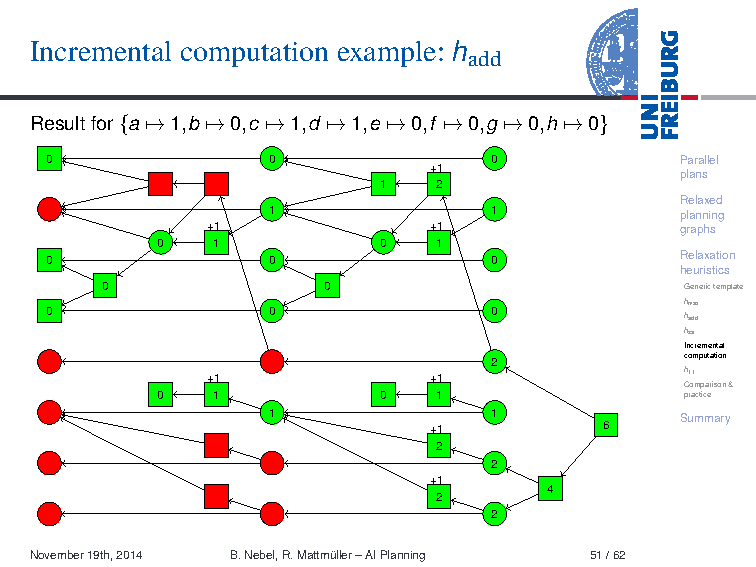
\includegraphics[scale=1]{aip08-handout51}
\end{figure}
=======
Date: & 05.12.2014\\
Students: & Axel Perschmann, Tarek Saier
\end{tabular}

\section*{Exercise 6.1}

\section*{Exercise 6.2}
$\Pi = \langle A,I,O,\gamma \rangle$ with\\
$A = \{a,b,c,d\}$\\
$I = \{a\mapsto 0,b\mapsto 0,c\mapsto 0,d\mapsto 0\}$\\
$\gamma = a\lor (b\land c\land d)$\\
$O=\{o_1,o_2\}$\\
$o_1=\langle \top, b\land c\land d\rangle$\\
$o_2=\langle b, a\rangle$\\
\\
\begin{tabular}{l} % to force the text part and the graph to appear on the same page
Relaxed planning graph with depth 3. (Sparse labeling due to technical restrictions.)\\
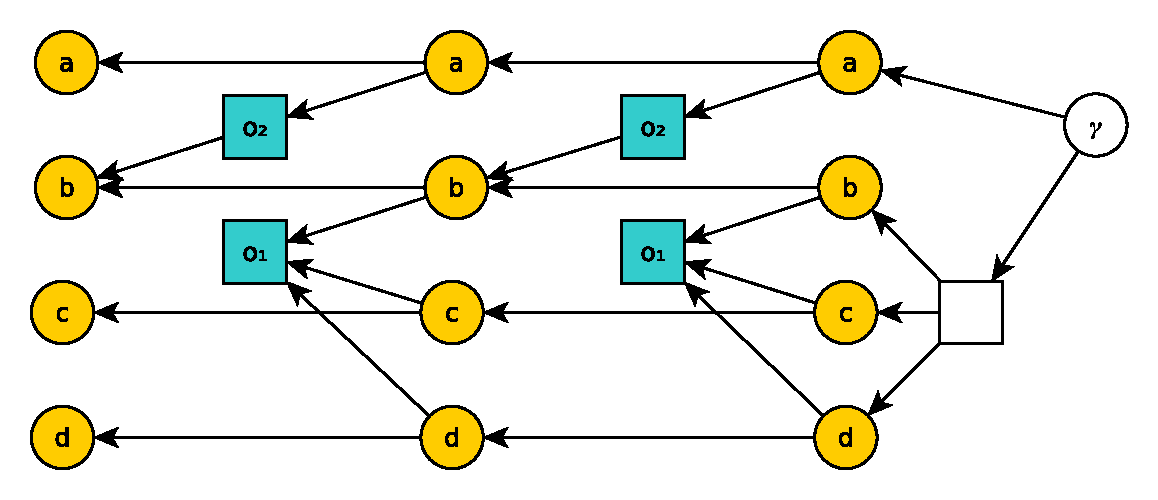
\includegraphics[scale=0.5]{g62}\\
\end{tabular}\\

\begin{tabular}{l} % to force the text part and the graph to appear on the same page
Depth 2, $h_{add}(I)=3$\\
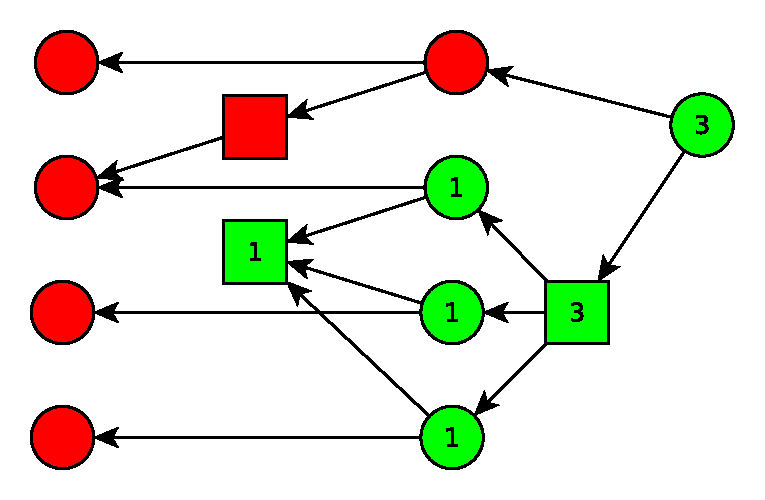
\includegraphics[scale=0.5]{g622}\\
\end{tabular}\\

\begin{tabular}{l} % to force the text part and the graph to appear on the same page
Depth 3, $h_{add}(I)=2$\\
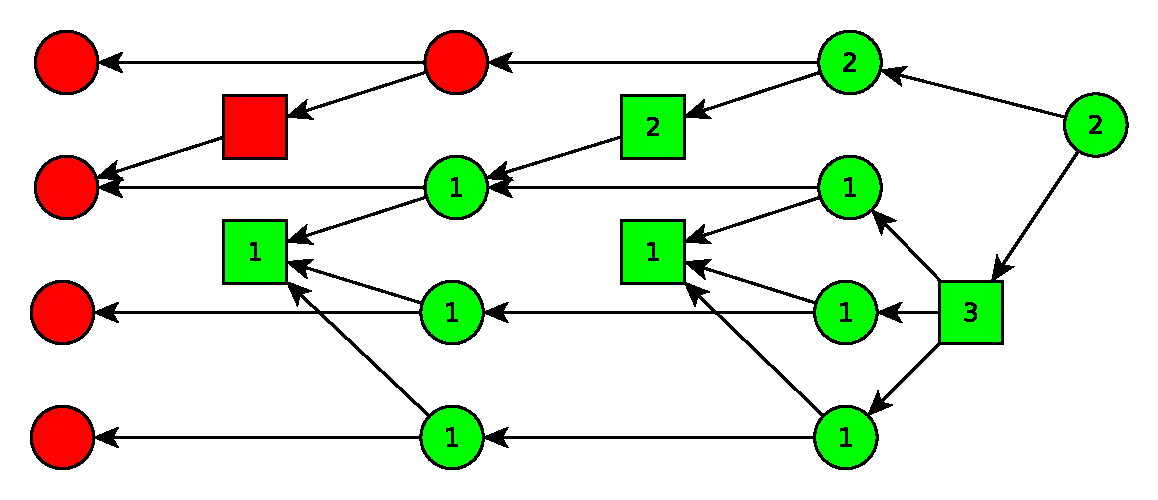
\includegraphics[scale=0.5]{g621}\\
\end{tabular}
>>>>>>> 82633ae9a0568e9ebdf3e2ef1195b4fdc92abcfd

\section*{Exercise 6.3}
\begin{tabular}{l} % to force the text part and the graph to appear on the same page
Relaxed planning graph with depth 3. (Sparse labeling due to technical restrictions.)\\
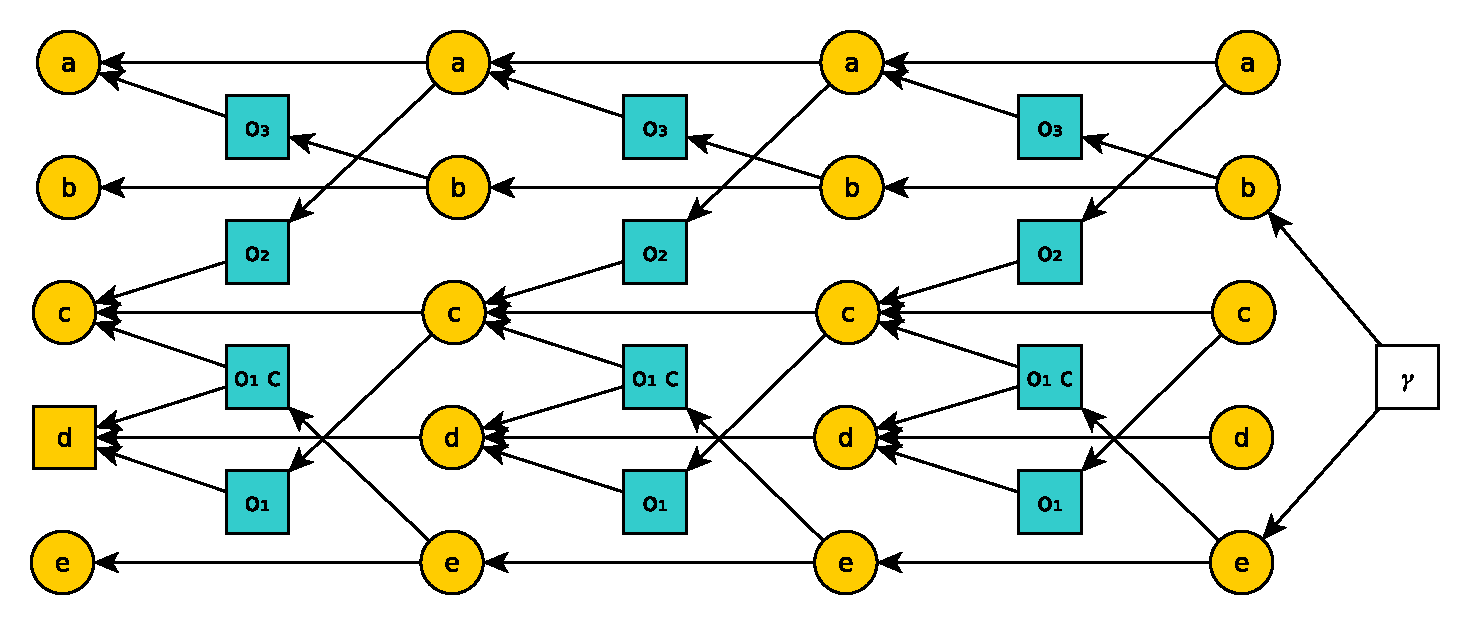
\includegraphics[scale=0.5]{g63}\\
\end{tabular}

\begin{tabular}{l} % to force the text part and the graph to appear on the same page
\textbf{(a)} $h_{max}(s)=3$\\
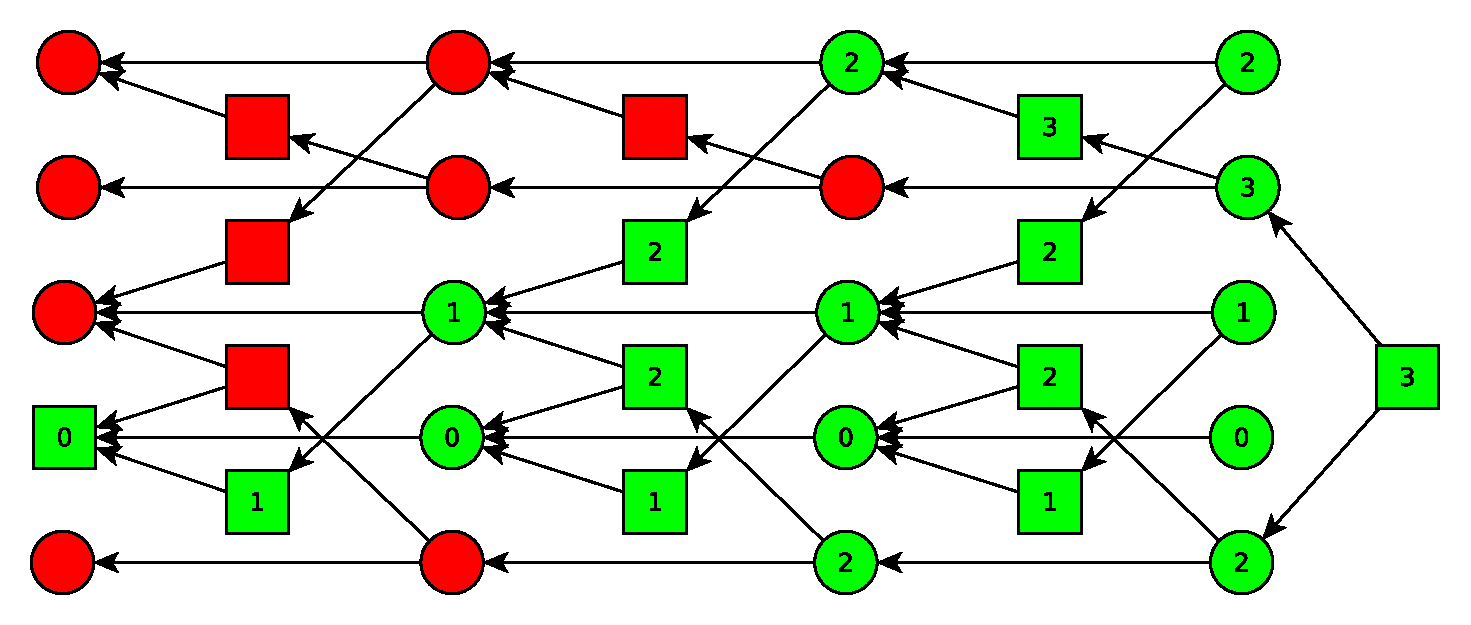
\includegraphics[scale=0.5]{g63a}\\
\end{tabular}

\begin{tabular}{l} % to force the text part and the graph to appear on the same page
\textbf{(b)} $h_{add}(s)=5$\\
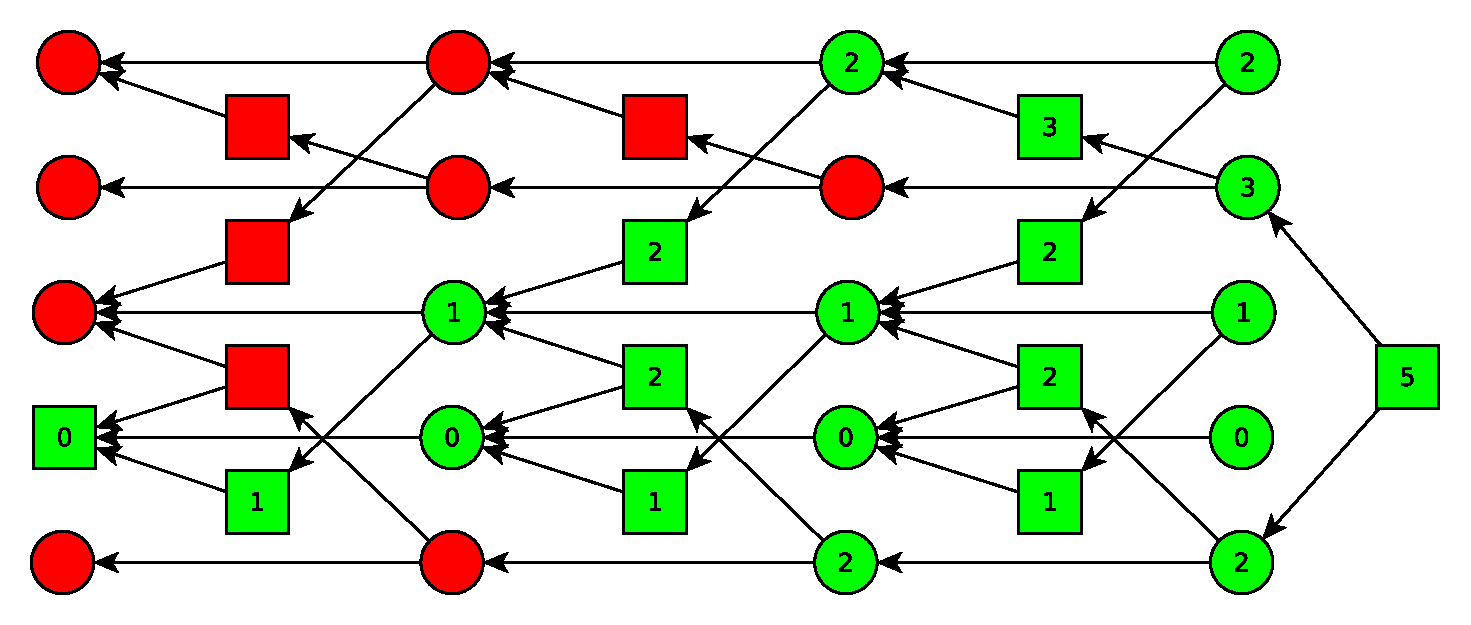
\includegraphics[scale=0.5]{g63b}\\
\end{tabular}

\begin{tabular}{l} % to force the text part and the graph to appear on the same page
\textbf{(c)} $h_{sa}(s)=4$\\
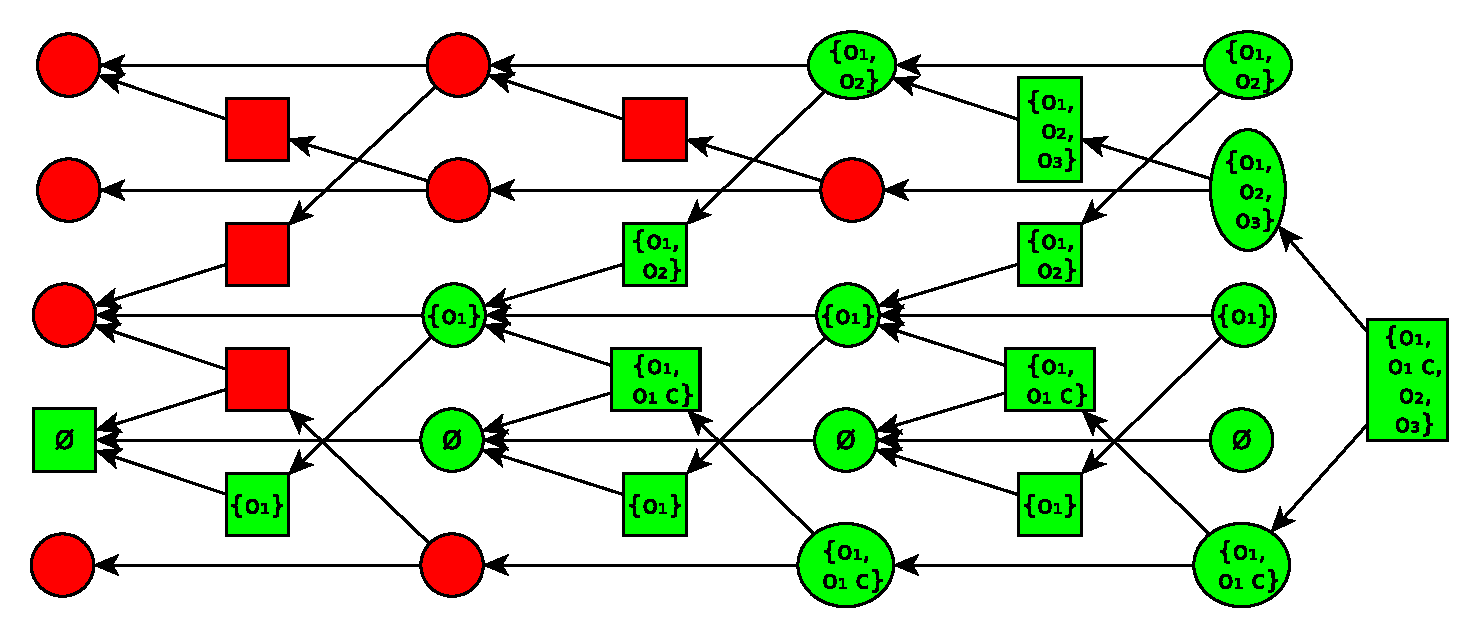
\includegraphics[scale=0.5]{g63c}\\
\end{tabular}

\begin{tabular}{l} % to force the text part and the graph to appear on the same page
\textbf{(d)} $h_{FF}(s)=4$\\
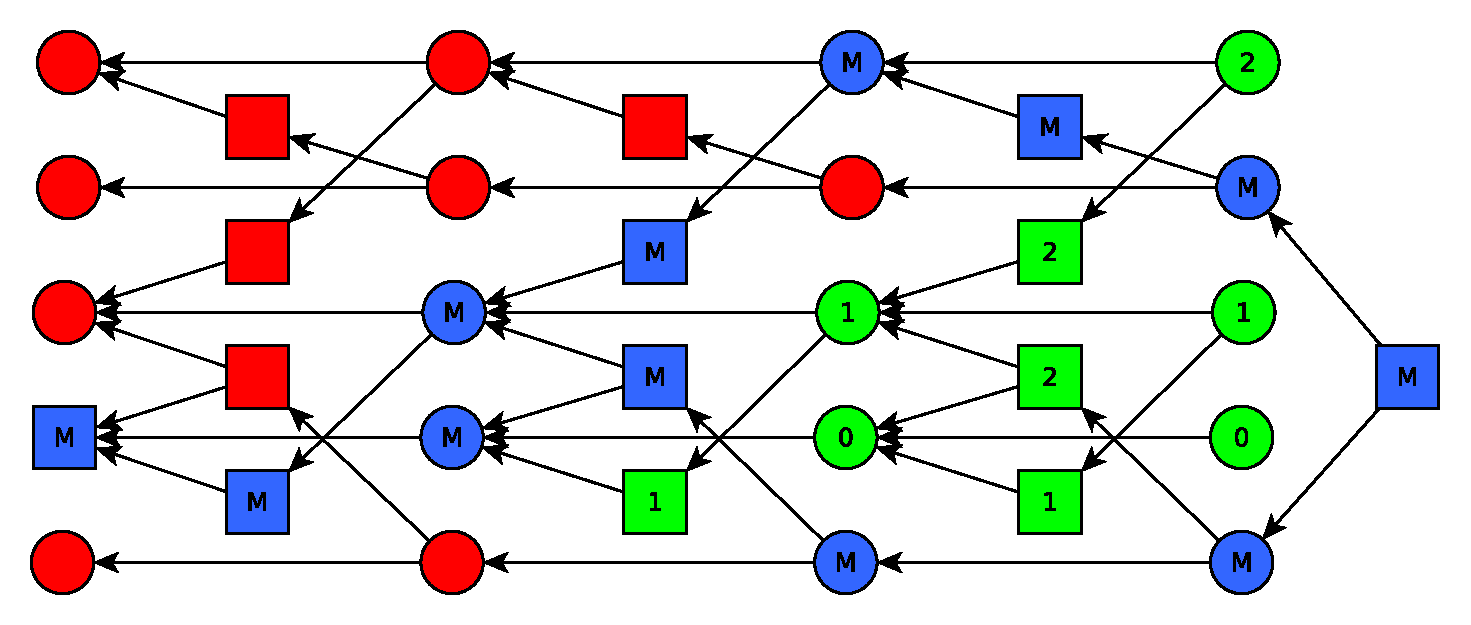
\includegraphics[scale=0.5]{g63d}\\
\end{tabular}


\section*{Exercise 6.1}


\end{document}
